\documentclass{article}
\usepackage[utf8]{inputenc}
\usepackage{fancyhdr}
\usepackage{pdflscape}
\usepackage{tabularx}
\usepackage{multicol}
\usepackage{setspace}
\usepackage{caption}
\usepackage{graphicx}
\usepackage{enumitem}
\usepackage{float}
\graphicspath{ {images/} }
\usepackage[style=authoryear,maxcitenames=2,dashed=false,backend=biber]{biblatex}
 \addbibresource{references.bib}
  \renewcommand*{\nameyeardelim}{\addcomma\space}
  \DeclareNameAlias{author}{last-first}
\pagestyle{fancy}
\fancyhf{}
\fancyhead[L, LO]{16COD292 | Project Initiation Document}
\cfoot{\thepage}

\title{Project Information Document}
\author{Matthew Elphick, Michael Fiford, Dhanesh Mistry}
\date{November 2016}
\begin{document}

\begin{titlepage}
\begin{center}
\textbf{\textsc{\Huge Project Initiation Document}}
\par
\vspace{0.5cm}
\textsc{\huge 16COD292}
\vfill
\textsc{\Huge Loughborough University}
\vspace{1cm}
\par
\textsc{\huge Matthew Elphick - B218391}
\par
\vspace{0.2cm}
\textsc{\huge Michael Fiford - B222639}
\par
\vspace{0.2cm}
\textsc{\huge Dhanesh Mistry - B219513}
\vspace{1cm}
\par
\textsc{\Huge 2016}
\end{center}
\end{titlepage}

\maketitle

\tableofcontents
\newpage

\begin{spacing}{2}
    \begin{center}
        \textsc{\huge{Atos IT Challenge - Blockchain}}
    \end{center}
\end{spacing}

\section{Introduction}


\subsection{Blockchain}

The theme for this year's Atos IT Challenge is \emph{Blockchain}. \textcite{cioblockchain} defines Blockchain technology as ``...a data structure that makes it possible to create a digital ledger of transactions and share it among a distributed network of computers.". Blockchain technology is fundamental to Bitcoin, a widely recognised cryptocurrency, as well as every other digital currency that has been spawned from Bitcoin's success. The technologies defining Blockchain have been identified by companies, and even governments, as a potentially disruptive, revolutionary, innovation \parencite{ukdlt, nomura_research_institute_survey_2016}.

\par

Blockchain provides a number of key features \parencite{blakemorganblockchain}:
\begin{itemize}
    \item Recorded, immutable history
    \item Trust without the need for trusted third parties
    \item Accountability
    \item Transparency
    \item Privacy
\end{itemize}

These features have recently made Blockchain a critical technology for the development of electronic currencies, however Blockchain is now being leveraged for a range of other applications for which its features can be utilised.

\subsection{Idea}

The subject of our project is Online Electronic Voting using Blockchain. Blockchain offers the opportunity for truly secure, anonymous online voting platforms, whilst being transparent and independently verifiable. Such a system has not been possible in the past, without Blockchain. Using traditional online application frameworks involving databases and private servers requires trust in one or more third-parties. Voters cannot be sure that their vote has been counted, unchanged, and not duplicated. Using a public ledger anyone will be able to count the results of a vote, as well as verifying that no person has voted more than once. Voters will also be able to look for their vote in the pool, whilst, thanks to Blind Signatures, no one else will be able to tell that their vote belongs to them.

\subsection{Client \& Users}

An online Blockchain voting platform is appealing to many potential clients, offering trust, security, and efficiency. Trade Unions, companies, and governments will be able to save thousands, or potentially millions, that would previously be spent on paper based systems and external third-party verification of their processes. The cost of the EU referendum was estimated by The Cabinet Office to be £142.4 million \parencite{eurefcost} which can be directly attributed to delivery by Royal Mail and counting of the votes. Such a platform will also allow parties to avoid potential issues associated with a physical paper system, such as the postponing of the Austrian presidential election in 2016 due to an issue with the adhesive seals on postal votes \parencite{Austrian41:online} or the fear of the votes themselves being lost or changed such as with the EU referendum \parencite{Thousand11:online}. Employees and customers of these clients would benefit from ease of use, proxy voting and the ability to verify the results.

\par

One example of such a use case would be for Trade Unions. Many facets of a union are controlled through voting, including their recognition by the Central Arbitration Committee if needed, \parencite{Employer56:online} and to the election of their key members \parencite{uktradeuni:online, Tradeuni41:online}. These votes involve many arduous arrangements by all involved and place a number of obligations on the unions themselves. A key part to this is the involvement of an independent party, the scrutineer, who manages the voting and produces a report on the result. Unions must wait for the scrutineer's report before publishing any results, and must also send out this report to all of their members. Once the scrutineer has been selected, every member must be informed of their name. The union members are then sent ballot papers by post, which they fill out and return, also by post \parencite{uktradeuni:online}. Similarities can be seen between this and the EU referendum, namely the large reliance on mail services, chiefly for sending and receiving votes and vote associated information, such as the scrutineers report, as well as the subsequent costs involved, which fall solely on the union as its members must be able to vote without any direct cost to themselves \parencite{uktradeuni:online}. Another issue that an electronic Blockchain voting system would address is the cost of the scrutineer, as well as the delay they introduce to the system in the production of their report. With Blockchain the results of the voting could immediately be available for the members to access and verify, and there would be no extra circulation cost or time delay incurred.

\par

Our company plans to sell Blockchain voting to these clients, offering both installation and hosting options. Hosting internally or with established firewalls would help affirm the security of the system. Once setup, the product should be self sufficient, offering options to create new polls, and manage user base, potentially supporting existing enterprise systems such as Windows Admin Tools. Pricing plans will limit the number of users, or number of polls. Companies can then choose to upgrade their package if they like the product. 24 Hour support should also be provided, to remotely assist enterprise clients should they run into any issues, for an additional cost. It could also be possible for prospective enterprise customers to download and test a public version of the app, to see if it fulfils their needs.

\par

The user facing application should be intuitive to use and not require specialist training. However help screens will be provided to help anyone that may struggle to use the application, such as in the potential case of lacking necessary computer literacy. This would provide an economic benefit to clients, saving them time and money which they would usually have to invest in a full training and support programme.

\subsection{Our Team}
\label{section:team}

\begin{description} % I tried to make this nicer with alignment and it messed up
\item[Matthew Elphick] Computer Science Masters student with experience in C\#, PHP, Ruby, and JavaScript both client side and server side with Node.js. Did a placement as a Software Engineer at Clock limited, a digital agency, building Node.js and PHP websites for clients.
\item[Michael Fiford] Computer Science Masters student with experience in C\#, Java, PHP and JavaScript. Completed a placement year at BAE Systems working on application testing, requirement verification, test automation, application prototyping and human computer interaction.
\item[Dhanesh Mistry] Computing \& Management Masters student with experience in C\#, ASP.NET MVC, PHP and JavaScript. During his placement year Dhanesh worked as a Junior Web Developer at Dignity Plc where his primary responsibility was to work on the migration of the company's corporate website to bring it in-house.
\end{description}

\section{Project Plan}

\subsection{Gantt Chart}
%A3 Gantt Chart in Appendix
A Gantt chart for the project has been included in the appendix of this document.
\subsection{Team Roles}

As noted in Section \ref{section:team}, this team consists of three members from two different Computer Science courses. The technical tasks are likely to be taken on by Matthew and Michael due to their background in software development with their respective placements and academic past, whereas Dhanesh will be primarily working on making the business case for the product due to the insight provided from the management focused sections of his degree. However, all members of the team are capable of taking on both technical and non-technical tasks, so the idea will be to allocate tasks based on team member strengths, but when required, assistance and time can be managed to complete all tasks, throughout the duration of the project.

\subsection{Team Responsibilities}
The following will outline the responsibilities for each member of this team. The responsibilities for the three members of the team are only intended as a rough guideline; it is expected that these responsibilities will change and be shared throughout the project as required.
\begin{description}
    \item[Matthew Elphick]
        \
        \begin{itemize}
            \item Development of the front-end GUI for the application.
            \item Development of controllers and layouts to interact with back-end API.
            \item Design of User Experience (UX) for the application.
            \item Development of an appropriate interaction layer to handle input/output of user and the system for the UX.
            \item Testing of front-end interaction with the back-end.
            \item Testing of front-end from a usability perspective. 
            \item Capture video content.
        \end{itemize}
    \item[Michael Fiford]
        \
        \begin{itemize}
            \item Development of back-end functionality of the system.
            \item Development of API for interaction with the front-end.
            \item Development of functionality to interface the Blockchain system.
            \item Development of the cryptographic algorithm for the encryption of the system.
            \item Testing of all aspects of the back-end functionality.
            \item Testing of Blockchain interface.
            \item Testing of interaction between API and front-end.
            \item Edit and transcode video.
        \end{itemize}
    \item[Dhanesh Mistry]
         \
        \begin{itemize}
            \item Development of the business case for the service.
            \item Production of any supporting documentation required for the application.
            \item Maintenance of social media presence of the team.
            \item Liaison between client from Atos and the team.
            \item Organisation of any group meetings both physical and remote.
            \item Tracking overall system development progress.
            \item Testing of overall system.
            \item Plan video content.
        \end{itemize}
\end{description}

\subsection{Milestones}
This section outlines the project milestones that we have identified as being imperative to the completion of this project. Some of these have been imposed by the module leader, and others by Atos, as deadlines for certain pieces of work to be submitted. There are future deadlines outlined by Atos that do not have a definite date at this moment in time \parencite{atosrules}, therefore the project plan will be updated accordingly once these come to light. Furthermore we have created our own milestones throughout the progression of the project to ensure that the progress runs smoothly.
\\
\\
Milestones imposed by Atos \parencite{atosrules}:
\begin{itemize}
    \item Registration of team on Atos IT Challenge website: \textbf{30th November 2016}.
    \item Submission of Idea: \textbf{30th November 2016}.
    \item Development of Solution: \textbf{December 2016 - April 2017}.
    \item Presentation of Solution to Atos: \textbf{May 2017}.
\end{itemize}
\ \\
Milestones imposed by module leader:
\begin{itemize}
    \item Submission of Final Report: \textbf{18th May 2017}.
\end{itemize}
\ \\
The team itself has also put forward some internal tentative milestones that we will aim for. These milestones are currently without a date, and will be added to the project plan once work has begun.
\\
\\
Milestones imposed by ourselves:
\begin{itemize}
    \item Working interface between Blockchain and Desktop Application.
    \item Initial Application Prototype.
    \item Second Prototype with Improvements from Clients.
    \item User Testing Completed.
    \item Completed Application.
    \item Completed Product Video.
\end{itemize}
\section{Literature Review Outline}

\subsection{Public Bodies and Blockchain}

There is an increasing trend of public bodies across the world adopting Blockchain technology, more-so the distributed ledger aspect of the technology.
\par
\textcite{dubaichain} explains how the government of Dubai wishes to use Blockchain technology for government documents. \textcite{dubaichain2} expands on this by saying that this is just part of an overall strategic plan where the endgame is to create a Blockchain platform for government services which could be opened up to other countries and cities in the future. 
\par
\textcite{auzchain} reported on how the Australian Postal Service wishes to provide an electronic voting service based on Blockchain technology. The Australia Post State Director for Victoria and Tasmania stated that ``using the Blockchain for voting would allow for a location agnostic, ``tamper proof" system that would provide traceability, prevent manipulation, yet allow anonymity, and be resistant to denial of service attacks." \parencite{auzchain}. These factors outline the security aspect of the Blockchain technology which would be paramount to any voting system that is eventually produced.
\par
Estonia has been overhauling its government services as of late in order to provide various services to its citizens digitally \parencite{estoniaeresidency}. These services include establishing and running a company online, gaining access to international payment providers and to be able to declare your taxes online \parencite{estoniaeresidency}. These services are all provided on the platform called ``e-residency" \parencite{estoniaeresidency}. One component of e-residency is the ability digitally sign legal documents such as birth certificates and business contracts and this is where Blockchain comes in. \textcite{estoniachain} is a Blockchain based digital governance platform and in 2015 they were selected to provide a public notary service for residents registered on the e-residency platform. \textcite{estoniachain} cites that ``distributed and immutable nature of this public notary makes it more secure than any notary currently offered by traditional nation states." This means that signatures of the notary can be verified independently and it prevents changes being made so this is perfect for giving residents the ability to digitally sign their own legal documents.
\par
As part of the Blackett review by the Government Office for Science, a report into Distributed technology was released outlining ways in which the UK Government could maximise the use of this technology to provide services in both public sector and the private sector \parencite{ukdlt}. Sir Mark Walport, the UK Government Chief Scientific Adviser explains how distributed ledgers could eliminate the risk of a centralised storage as a central point of failure \parencite{ukdlt2}.
\par
Overall these cases show that there is an increasing amount of public bodies across the world that are looking into the adoption of Blockchain technology. However the focus here seems to be mainly on the distributed ledger technology that underpins the Blockchain rather than the aspects used for a digital currency, citing how Blockchain can allow for anonymity and traceability whilst being in a distributed system eliminating the need for a central storage point. Furthermore in Dubai's case they are willing to go as far as to digitising all government documents and even providing a platform that can be distributed to other countries.

\subsection{Blockchain and The Private Sector}

With the advent of Blockchain technology and Bitcoin, there are an increasing amount of companies within the private sector grasping the technology to perform various tasks that were not feasible in the past without Blockchain.
\par
Recently EY, a consultancy company, formed a partnership with The Bitfury Group where Bitfury will provide Blockchain services to EY which in turn allows EY to provide Blockchain-based solutions to their clients \parencite{eyblockchain}. \textcite{eyblockchain} explains that this deals could mean that Blockchain-based solutions may start to appear in different sectors beyond the finance sector. This shows that there is scope for the underlying technology behind Blockchain to be utilised in a non-financial organisation whereby the services provided are not part of a financial product.
\par
Verizon, the American telecommunications company has considered using Blockchain technology as a form of digital rights management platform \parencite{verizonblockchain}. \textcite{verizonblockchain} explains that Verizon has the issue of managing masses of customer data, especially across different borders. They can use Blockchain to provide users with a secure method of accessing their services and to manage information held within their systems. \textcite{verizonblockchain} goes on to say that due to the decentralisation of data, Verizon can potentially save on the costs of maintaining a large central database and servers with associated costs regarding the staffing required to verify and authorise transfer of data. This shows that not only can Blockchain be used to streamline digital rights management and management of customer data but can also bring about cost savings due to a lesser dependence on centralised databases and server hardware.
\par
The German energy company RWE has partnered with Slock.it, a smart contract system based on Blockchain, in order to develop a way to charge electric cars autonomously \parencite{rweblockchain}. \textcite{rweblockchain} explains that cars would essentially possess digital wallets that allows them to communicate with the car charging stations. These would utilise smart contracts in order to charge the car autonomously with a refundable deposit taken as security. Stephan Tual, the COO of Slock.it explains that the Blockchain acts as a secure entity between the charging station and the car so this functionality needn't be dependent on one car manufacturer \parencite{rweblockchain}. \textcite{rweblockchain} outlines that this could have various applications such as charging pads under traffic lights. This shows that the secure nature of Blockchain technology can act as authorisation to many services across a range of fields and differing technologies, not just computing.
\par
In general these cases explain that there are various use cases and applications for Blockchain technology and despite the emphasis of Blockchain being used in the financial sector, increasingly there are solutions coming forward that are not related to financial products and services, such as the solution being considered by Verizon.

\subsection{Blockchain and Voting}

As previously mentioned Blockchain technology offers a number of benefits many of which, such as a recorded immutable history, trust, and transparency, can be leveraged for use in online voting. Another benefit, independent to Blockchain itself, would be that electronic voting is hoped to improve voter turnout, resulting in improving the representation for any vote \parencite{bchainpres:online}. However `traditional' electronic voting faces many issues, which Blockchain enables implementations to overcome. There has recently been significant interest in combining voting and Blockchain, with a lot of investment in the area \parencite{CoinDesk73:online, CoinDesk42:online}.
\par
One approach to bringing together the idea of voting and Blockchain is using voting as a core idea to the Blockchain itself, such as in the case of the Tezos Blockchain implementation which implements voting from the start of the chain using voting to reach consensus about the state of the chain, as well as voting by participants on how the very protocol itself and its nodes should adapt and upgrade. \parencite{TezosAse64:online}. 
\par
The more common approach is to use existing Blockchain implementations to build platforms for voting. The level of such voting platforms varies wildly, with Blockchain being suggested and considered for use by businesses and investors \parencite{Delaware81:online}, to the likes of governments and parliaments \parencite{USPresid50:online, CoinDesk74:online}. Indeed a topical example would be the 'Ballot Box' concept that SettleMint put together for the 2016 Presidential Election which uses Blockchain and associated technologies \parencite{USPresid50:online}. While only the working concept is available at the moment SettleMint have said that they will release a white-paper soon on the implementation of this application \parencite{SettleMi18:online}, which will be of interest to look in to and use for inspiration and guidance for our own voting platform.

\subsection{Cryptography}

Cryptography is the cornerstone of any online voting application. Many systems, for example UK Elections, operate on a `Secret Ballot' system, where voter's choices are protected through anonymity \parencite{chartistssecretbalot:online}. It is important to protect these philosophies despite the change of voting medium. To do so various cryptographic techniques must be implemented correctly.

\subsubsection{Asymmetric Cryptography}

This cryptographic technique, also commonly known as `Public-key Cryptography', relies upon a `trapdoor function', where the result of an operation is easy to calculate, but hard to reverse \parencite{trapdoor}. \textcite{trapdoor} theorised that such a technique could be used with asymmetric keys for secure exchange of messages without the need for secure key exchange. This was later implemented by \textcite{rsa} in the form of RSA. Alternative algorithms for asymmetric cryptography also exist, such as DSA \parencite{dsa} or elliptic curve cryptography \parencite{ecc}, offering benefits such as reduced key size and increased computation difficulty. Many of these techniques also provide signing algorithms, using key-pairs, providing verification and immutability \parencite{rsa, dsa, ecc}.

\subsubsection{Blind Signatures}

Blind signatures are an extended variation, with a key difference from regular signatures: the original message is not known by the party signing the message \parencite{blindsignatures}. This could be implemented to create an untraceable payments system, or provide anonymity in a voting platform such as the proposed system. The user can irrefutably prove that another party (authority) has signed their message. One popular implementation of blind signatures, RSA, uses the equation \parencite{blindsignaturersa}:

\begin{equation}
s' = (M')^d = M^d . (r^e)^d = M^d . r \pmod N
\end{equation}

Where $M$ is the message being sent, $N$ and $e$ are publicly known values, and $d$ represents the secret information of the signer, obtained from the inverse of $e \mod \phi(n)$. $r$ is a random relative prime known only to the client.

\section{Software Development Approach}

Due to the small team size of only 3 members, with only 2 of those heavily contributing directly to the development process itself, a simplified software development methodology will be undertaken. Ultimately many of the principles seen in the Agile approach can be utilised in this project, and are especially relevant as we have fixed resources and time but only an estimate of what the features will be.
\par
Some key ideas that can be taken from Agile are that the produced software should be our primary measure of progress, and that the main approach for development should be to iteratively create new features, gain feedback from the client and continuously improve the product \parencite{agilemanifesto, layton2012agile}. However in this case the client will be a mixture of the team members themselves, as well as Dr Christian W Dawson and members at Atos. This will allow us to produce a good product for the Atos IT challenge by garnering opinions which we can respond to and should ultimately allow us to maximise the benefit for the end-users and business partners, as well as the look and feel of the product itself, all key parts of the challenge \parencite{atosrules}. We will also use the Kanban method to keep track of and allocate development tasks, allowing each individual to become more self-autonomous within the team. This method is discussed more in Section \ref{projectmanagementref}.

\section{Risk Assessment Plan}

There are many risks that are associated with a project of this nature. A risk assessment plan is required in order to help alleviate the effects these risks have to the progression of this project.

\subsection{Methodology of Assessing Risk Impact}

For assessing the impact of the risks of this project, we will use the formula outlined by \textcite[][84]{dawson15}:
\begin{equation}
Risk Impact = Likelihood * Consequence
\end{equation}
For the scoring measures of both risk likelihood and risk consequence, \textcite[][85]{dawson15} makes reference to \textcite[][256]{turner93} which devises scores:

\begin{multicols}{2}
    \begin{center}
    
        \vspace{0.1cm}
        \centering
        \begin{tabular}{|c|c|} \hline
            \textbf{Risk Likelihood} & \textbf{Score} \\
            \hline
            Low & 1 \\ \hline
            Medium & 2 \\ \hline
            High & 3 \\ \hline
        \end{tabular}
    \end{center}
    
    \begin{center}
        \vspace{0.1cm}
        \centering
        \begin{tabular}{|c|c|} \hline
            \textbf{Risk Consequence} & \textbf{Score} \\ \hline
            Very Low & 1 \\ \hline
            Low & 2 \\ \hline
            Medium & 3 \\ \hline
            High & 4 \\ \hline
            Very High & 5 \\ \hline
        \end{tabular}
    \end{center}
\end{multicols}

\begin{multicols}{2}
    \captionof{table}{Risk likelihood scores}
    \captionof{table}{Risk consequence scores}
\end{multicols}

\par
\subsection{Method of Control}
There are several ways in which to control risk management. \textcite[][87]{dawson15} suggests three methods of managing risks:
\begin{description}[labelindent=\parindent]
    \item[Contingency] - This is essentially creating a backup plan so that the risk damage is reduced.
    \item[Deflection] - This involves finding an alternative to a problem in order to reduce the impact of the risk.
    \item[Avoidance] - This is where the risk itself is avoided altogether.
\end{description}
We will use these categories to assist in controlling the impact of all risks that have been identified in the project.
\par

\subsection{Plan}

Based on the defined methodology, Table \ref{table:risks} outlines the risks associated with the project, their impact levels, and the actions that will be taken to help reduce the impact of these risks.
\newpage
\begin{landscape}
\begin{table}[ht]
    \caption{Risk Assessment Plan}
    \label{table:risks}
    \centering
    \begin{tabularx}{\linewidth}{|X|X|X|X|X|X|} \hline
    \textbf{Risk} & \textbf{Risk Likelihood} & \textbf{Risk Consequence} &\textbf{Risk Impact} & \textbf{Method of Control} & \textbf{Measures Taken to Control Impact} \tabularnewline
    \hline
    Computer Hardware Failure & 1 & 4 & 4 & Contingency & Desktops at home or lab computers available at the University can be used to continue working on project. \\ \hline
    Loss of Application Code & 2 & 4 & 8 & Avoidance & Application code is backed up in cloud Git repository and can be restored when required. \\ \hline
    Loss of Supporting Documentation & 2 & 4 & 8 & Avoidance & Supporting documentation is backed up in Dropbox or ShareLaTeX depending on type of documentation. \\ \hline
    Compatibility issues with Development Platform & 1 & 3 & 3 & Avoidance & Development platform will be chosen that is compatible with our computers. \\ \hline
    \end{tabularx}
\end{table}
\newpage
\begin{table}[ht]
    \centering
    \begin{tabularx}{\linewidth}{|X|X|X|X|X|X|} \hline
    Lack of Knowledge of Program Language & 2 & 3 & 6 & Avoidance & Common program language will be chosen that we all know and works best with the Blockchain system. \\ \hline
    Lack of Knowledge for a Software Solution & 2 & 3 & 6 & Deflection & Where possible we will look to use existing packages that resolve issues rather than code our own solution \\ \hline
    Team Member Illness & 2 & 3 & 6 & Contingency & Other members of the team can take on the responsibility should the situation arise. \\ \hline
    Failure of Hosting Platform & 2 & 4 & 8 & Contingency & Alternative hosting platform could be used or system could be self-hosted if required. \\ \hline
    Conflict with Other Work Commitments & 2 & 3 & 6 & Avoidance & Responsibilities will be set so that team members have enough time to complete them. \\ \hline
    Loss of Internet Connection & 2 & 4 & 8 & Contingency & Internet connection at university can be used if connection is lost at home and vice-versa. \\ \hline
    \end{tabularx}
\end{table}
\end{landscape}
\newpage

\section{Project Management}
\label{projectmanagementref}

To manage this project, we aim to take advantage of a variety of project management tools that will help us to efficiently control the various aspects of the project. 
\subsection{Communication}
\subsubsection{Slack}
For communication in this project we will be using Slack, a project communication and collaboration tool. Slack allows us to separate conversations into different ``channels" so that group conversations can be put into a specific topic area rather than getting lost in the overall conversation. In addition to this Slack allows for a range of services to be integrated into the platform to centralise a lot of the information about the team and work. For example there is a Google Calendar integration available where alerts are sent out whenever meetings are arranged and reminders are sent daily about any events for the day. Furthermore there is also a private chat function available should we wish to have a one-to-one conversation with another team member about any part of the project.
\subsubsection{Skype}
For meetings that we need to conduct off-campus, we will also be using Skype to host conference calls should we need to have more in-depth conversations about parts of the project as it progresses.

\subsection{Meetings}

We aim to hold regular meetings of some form at least once a week, more if required. This is dependent on our timetables and on any work schedules. Additionally two members of the team live off-campus so we would utilise Skype to hold remote meetings if required as previously mentioned. Typically these meetings will be scheduled in advanced and are held as appropriate to the task at hand.

\subsubsection{Meeting Structure}

The structure of the meetings themselves will heavily depend on the state of the project and the topic areas being discussed. This is the general meeting structure that we aim to follow:

\begin{itemize}
    \item Meetings will be arranged in advanced with date, time, and location recorded on an event in Google Calendar.
    \item Topic areas may also be decided on in advance but they can be subject to change.
    \item On start of the meeting, the role of the scribe is decided - this will typically rotate as there are only three members in this team.
    \item Once the scribe role has been assigned the plan of action from the previous meeting will be reviewed.
    \item There is no chairperson due to the relative small size of the team but should a situation arise, Dhanesh will act as adjudicator to help finalise certain decisions.
    \item Meetings should typically last for some time between 30 minutes to 1 hour, but once again this will depend on the subject matters being discussed.
    \item At the end of meetings, a plan of action is created with tasks to be carried out by all members with time-specific deadlines set depending on the task at hand.
    \item After the meeting  notes taken by the elected scribe will be uploaded to Slack where all team members can review proceedings as required.
\end{itemize}

Whilst the general structure has been set out, these meetings will be flexible in nature so discussions may not follow a specific agenda but rather cover topics that are deemed to be relevant and important at the time. We are inclined to hold these meetings regularly as this will provide us with an overall status update on the project which will help us to identify what we are doing well and what needs to be improved upon.

\subsection{Work Allocation}

Our team is relatively small as there are only three members. Nonetheless we still require a system of allocating tasks between members so that the work is evenly distributed and allocated based on the skills and relevant skill level of the team member as everyone is able to bring something to the team. 

\subsubsection{Trello}

For work allocation, we will be using a tool called Trello. Trello is a project management tool that uses the Kanban paradigm approach to management. There is one overall screen where all tasks can been seen, which are then categorised into separate boards. Typically the boards are categorised at statuses so that team members can identify the current state of the task at a glance, for example, `In Progress', `Testing' and `Completed'. Trello allows for tasks to be assigned to each member of a team and deadlines can be set for each task.

\par

Ultimately the Kanban approach featured in Trello provides several advantages, such as giving a visualisation of the work flow, allowing self organisation, collaborative improvement, and an experimental approach to projects as discussed by \textcite{anderson2010kanban}. These benefits ultimately mean that Trello lends itself both to this style of project, as well as to small teams such as our own \parencite{kanbanforasmallteam, whenkanbanworksbest}. Furthermore Trello can be integrated with Slack to send out alerts to all team members regarding the allocation and progress of all tasks of the project, and to help ensure that all team members are kept up to date.

\section{Technical Considerations}

\subsection{Blockchain}

Within Blockchain technology, there are still a number of options and differing opinions on how to approach certain issues.

\par

One such key issue is which consensus algorithm to use. This consensus algorithm is used by the Blockchain to resolve the current state of itself, such as the case of conflicting opinions about the state of the Blockchain, and to validate transactions. This is vital due to the architecture of Blockchain technology: while anyone can add to a Blockchain, we still only want one unique and final chain of transactions that we can trust. Here we will discuss two such algorithms that are used to allow the chain to do this.

\subsubsection{Proof-of-work}

The first approach is the proof-of-work consensus algorithm. This is the approach seen in Bitcoin, where to add to the chain members must \emph{mine} a block. This mining uses a real-world resources (computational time and electricity) to solve a complex mathematical problem \parencite{nakamoto2008bitcoin}. As such there's no way to cheat the system by either falsification or duplicated transactions, as you must have the correct solution to the correct problem the first time it is seen. In this way the longest valid chain which has had the highest amount of work put in to it can be chosen as the correct state of the entire chain. However this brings with it certain issues, namely that each full node of the network which 'mines' and contributes in some way requires substantial computing capacity proportional to the security requirements of the Blockchain network. This is generally inefficient and wastes a lot of energy and hardware purely to guarantee validity of the network. The proportional relationship between capacity and security is due to the fact that scarcity and validity of the currency/transaction cost is tied directly to these real-world resources. Therefore high security of the network can only be achieved at increased capacity of the network, subsequently meaning at high operating costs. Another potential issue with proof-of-work is that it may suffer from the market failure scenario of \emph{Tragedy of the Commons} from Game Theory \parencite{garrett_hardin_tragedy_1968, Iftxlimi23:online, economic46:online}. In such a scenario mining becomes so low in reward that there is minimal interest for each individual miner to continue to mine. This reduction in mining will lower the computing capacity of the network, and so too the security of the Blockchain network itself, opening it to attack, which is obviously against the interest of the Blockchain community as a whole \parencite{Bitcoinw83:online}. However it is worth noting that it is only conjecture that this issue may arise, and indeed the opposite Comedy of Commons \parencite{rose1986comedy} may occur.

\subsubsection{Proof-of-stake}

The second is the newer proof-of-stake consensus algorithm. In this algorithm, instead of your computational capacity you use to contribute to the network, your stake or 'share' in the networks transactions weights how you can state your opinion on the validity of the Blockchain and vouch for the validity of transactions \parencite{ProofofS99:online}. How this translates into the actual implementation is that each 'miner' in the network is instead treated as a 'validator'. Under a proof-of-stake system each validator node can 'bond' a stake, in other terms they can put forward collateral to vouch for a block. This means that the security is no longer tied directly to the capacity of the Blockchain network, but instead to the chain with the highest number of validators that can vouch for it. In this way each of the nodes has a 'stake' in the network they have vouched for being correct, least they lose their collateral. This changes what is invested in in the network, in proof-of-work the underlying Blockchain network and its capacity is invested in, while in proof-of-stake it is the transactions themselves. In this way proof-of-stake network can be expected to have a higher stability as that is in the best interest of all the individuals, while a proof-of-work network will be more liquid as each individuals interest will be in maximising their own share. A popular proof-of-stake algorithm proposal is the Casper implementation by Ethereum \parencite{friendlyghost}, the specification of which is still being written \parencite{caspaspecnotes}. In Casper, as well as losing the collateral, any validator which bonded anything eventually deemed to be invalid will also lose their rights to be included in the consensus of deciding what is and isn't valid to assist in preventing the issue of double spending \parencite{caspaspecnotes}.

\subsubsection{Use Cases}

Proof-of-work is the most widely used consensus algorithm, as it is the approached used in Bitcoin itself \parencite{nakamoto2008bitcoin}, and is also implemented in other Blockchain implementations such as MutliChain \parencite{MultiCha46:online}, and Ethereum \parencite{WhitePap68:online}. However proof-of-stake is beginning to take hold with Ethereum looking in to adding the Casper protocol \parencite{friendlyghost}, PeerCoin \parencite{WhitepapPPCoin:online}, Bitshares \parencite{WhitepapBitshares:online}, as well as entirely proof-of-stake based cryptocurrencies being developed such as Nxt \parencite{WhitepapNxt:online}.

\par

In the case of Electronic Voting the proof-of-stake consensus approach would be preferable due to a number of varying reasons. Proof-of-work works because each individual has a vested interest in increasing their own computing capacity as required by the network for the associated mining reward, however in the application of voting such an incentive does not exist. It would also be unreasonable to expect all the end users in an organisation to have access to sufficient computing capacity to be involved in the Blockchain as it grows. As such proof-of-stake is the natural preference as it is not tied to the computing capacity. As it is not tied to computing capacity proof-of-stake has the added benefit of having the possibility of being utilised on a mobile platform which would have sufficient computational power to be involved in the proof-of-stake based Blockchain \parencite{Blockcha72:online}. Proof-of-stake also has the added benefit that an attack of the network in a conventional proof-of-work manner, that is to say gaining control over the majority of the network, is substantially more expensive to perform, and not in the interest of the attacker as any attacks against a proof-of-stake network act to reduce trust in the network and subsequently devalue the stakes and so result in a loss for the entire network including the attacker \parencite{Blockcha72:online}.

\subsection{User Application}

We are still currently exploring the best framework and language to provide the user-facing application for a Blockchain voting platform. The current languages being considered are JavaScript in the form of Electron, and C\# in the form of .NET 4.6 Windows Presentation Format (WPF).

\subsubsection{Web vs Desktop Applications}

The only truly secure way to vote on Blockchain without trusting another party, is for the client to directly create their voting transaction(s) themselves. If the user does not do this themselves, and instead votes via a third-party, they are forced to trust one or more intermediaries between themselves and the Blockchain. A third-party could alter, track, or destroy a user's vote, ultimately undermining the main benefits of using Blockchain technologies. To allow their vote to be placed directly onto the Blockchain the client will need to run a `Full Node'. A Full Node means that all history (blocks) of the Blockchain needs to be downloaded, as well as processing all new transactions. This results in the user having to download and run the client on their machine, as opposed to an increasingly popular web-based application.

\subsubsection{Blockchain Size}

The size of the Blockchain on a user's system is something that needs to be considered, assessed, and carefully managed during the application development process. For example, Bitcoin has grown to nearly 90GB \parencite{blockchaininfosize}. The larger the number of votes, the larger the Blockchain will be.

\subsubsection{Operating System}

Whilst it would be desirable to have a cross-platform desktop application, given that our target audience is businesses,  we have identified that it would be acceptable to produce a Windows only platform, as a prototype and an acceptable first instance of our platform. Windows accounts for almost 90\% of Desktop Operating Systems \parencite{operatingsystemstats}.

\subsubsection{Trade-offs}

The choice of either one of these frameworks offers their own unique benefits, as well as suffering from some compromises. Benefits of Electron include: fast development, ease of styles using HTML and CSS, cross-platform functionality, and reuse of some of the application code for the API (Section \ref{section:registrar-api}). However, an associated compromises is that Electron/Node.js apps can get large with many dependencies which can be hard to manage and could result in wasted time. Additionally Electron apps require separation of the front and back-end code, resorting back to a form of the client/server paradigm, despite running on the same machine.

\par

If we choose to go with a C\# WPF application, we would lose out on all the benefits previously mentioned that we'd get with an Electron based application, which includes desirable cross-platform operability. However we would instead gain: application scaling, execution speed, data bindings and live debugging.

\subsection{Registrar API}
\label{section:registrar-api}

Separate from the Blockchain technologies, we have identified that an anonymous online voting system will require a `Registrar' in the form of an Application Programming Interface (API). Whilst this is partially against peer-to-peer nature of Blockchain itself, it is necessary to provide authorisation, and limitation. Without a Registrar, anyone could vote, and they could vote as many times as they like. In order for a vote to be counted as valid, it will have to had been cast using a token that has been blindly signed by the Registrar. The Registrar will also track who has been allocated a token, allowing strict control to number of votes, who can vote, and enforcing other commonly found voting regulations such as bans.

\par

Following convention, the API will most likely be web-based. Our team does not have easy access to any Windows servers, however do have access to a few Linux servers. Therefore we plan to to write a Node.js API, interfacing with the Blockchain, and providing authority over the voting process.

\section{Outline Ideas}

Included below are some rough initial ideas we have had for how the application will be used, as well as some drafted application layouts. Additionally, we have created the name `evoto' for our company. We plan to move forward with this as our Atos IT Challenge team name, using it for company advertising on social media and GitHub. Within the next few weeks we also hope to have designed an evoto logo to help identify our brand.

\begin{centering}
    \begin{figure}[H]
        \centering
        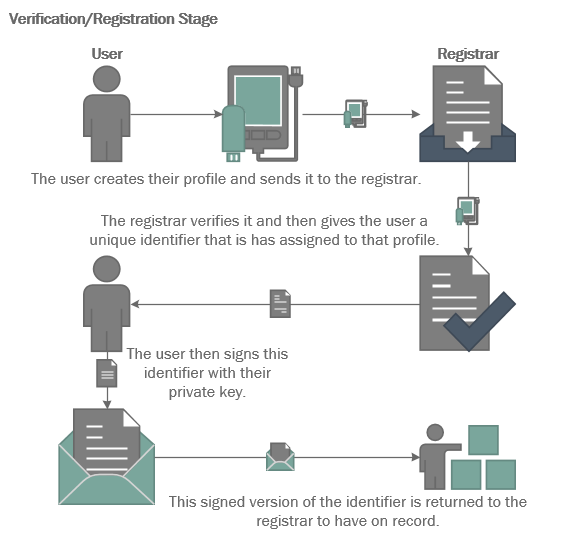
\includegraphics[width=0.9\textwidth]{verification}
        \caption{The proposed verification/registration steps.}
        \label{fig:registration}
    \end{figure}

    \begin{figure}[H]
        \centering
        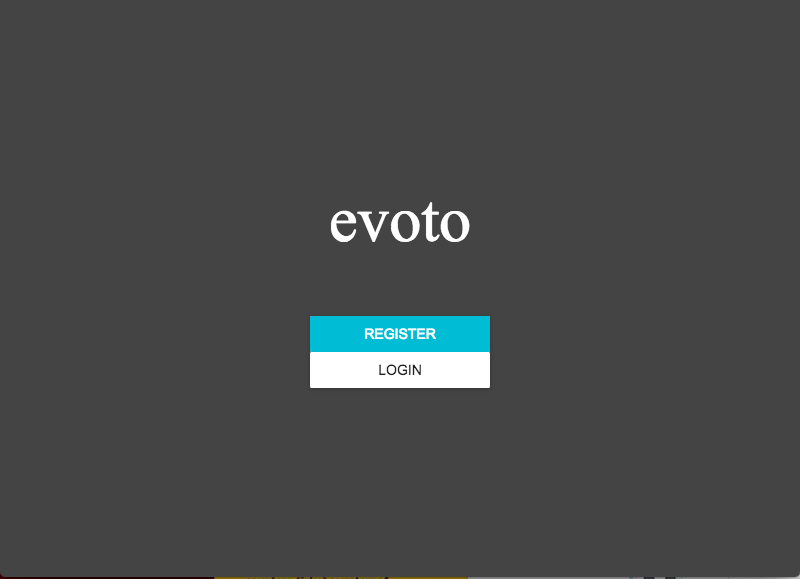
\includegraphics[width=0.9\textwidth]{screenshots/screen-start}
        \caption{The start screen for the desktop application.}
        \label{fig:registration}
    \end{figure}
    
    \begin{figure}[H]
        \centering
        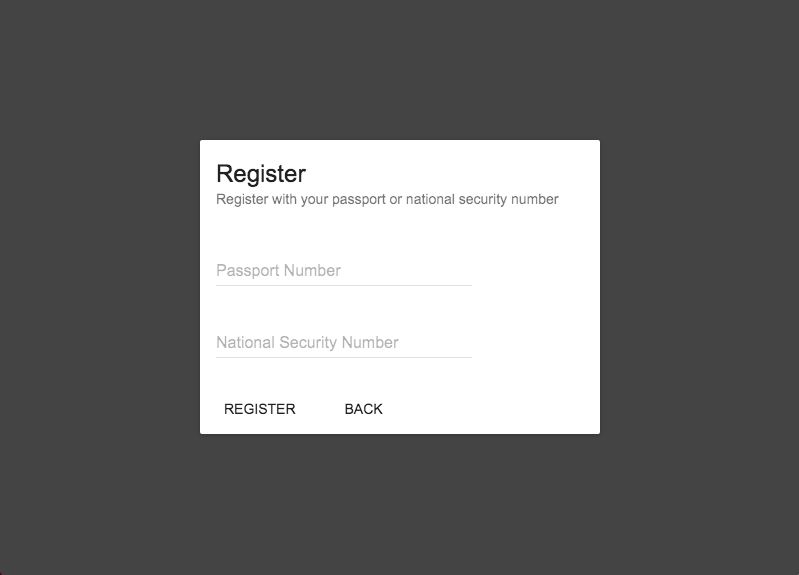
\includegraphics[width=0.9\textwidth]{screenshots/screen-register}
        \caption{The registration screen for the desktop application.}
        \label{fig:registration}
    \end{figure}
    
    \begin{figure}[H]
        \centering
        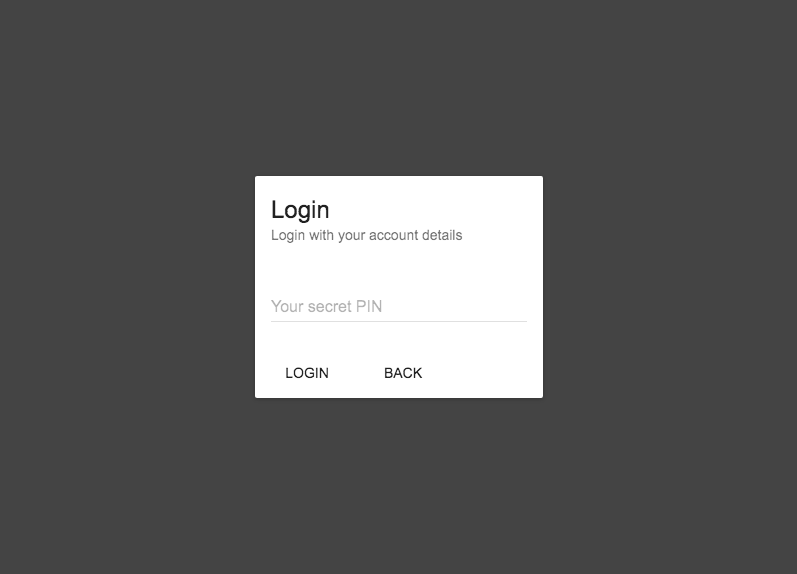
\includegraphics[width=0.9\textwidth]{screenshots/screen-login}
        \caption{The login screen for the desktop application.}
        \label{fig:registration}
    \end{figure}
    
    \begin{figure}[H]
        \centering
        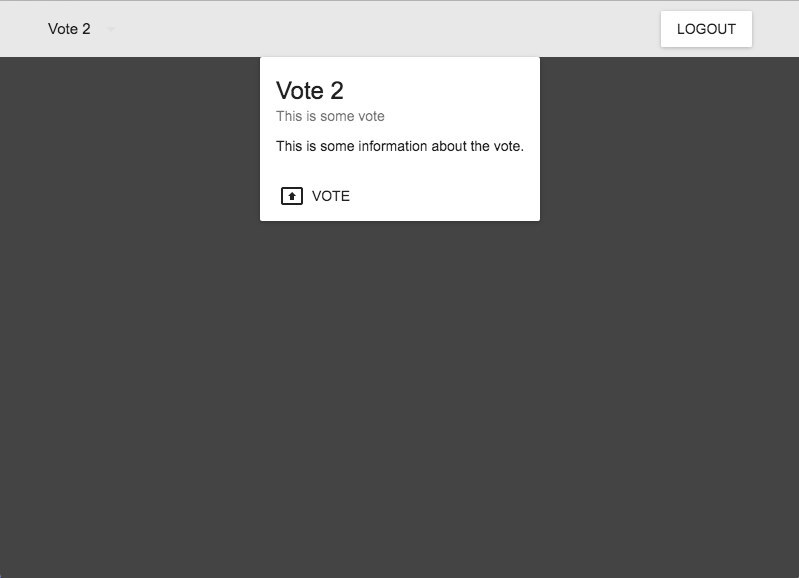
\includegraphics[width=0.9\textwidth]{screenshots/screen-vote-info}
        \caption{The vote information screen for the desktop application.}
        \label{fig:registration}
    \end{figure}
    
    \begin{figure}[H]
        \centering
        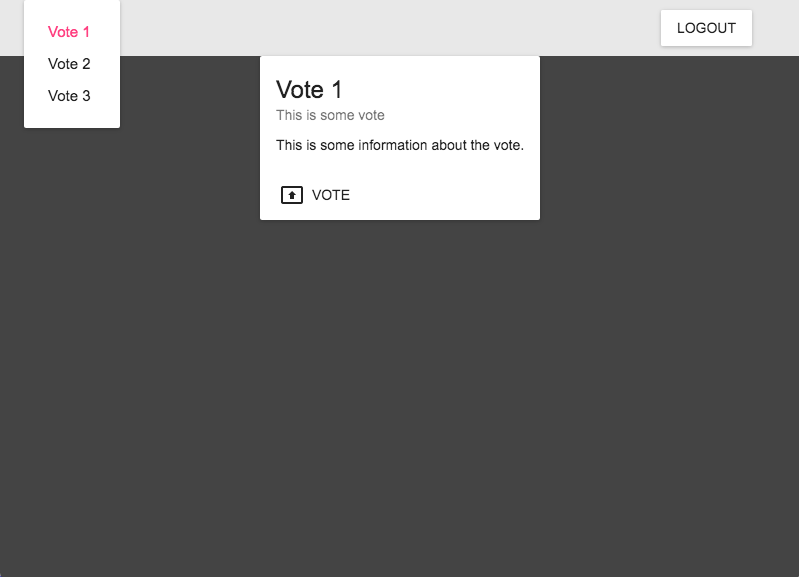
\includegraphics[width=0.9\textwidth]{screenshots/screen-vote-choices}
        \caption{The vote information screen with vote choices for the desktop application.}
        \label{fig:registration}
    \end{figure}
    
    \begin{figure}[H]
        \centering
        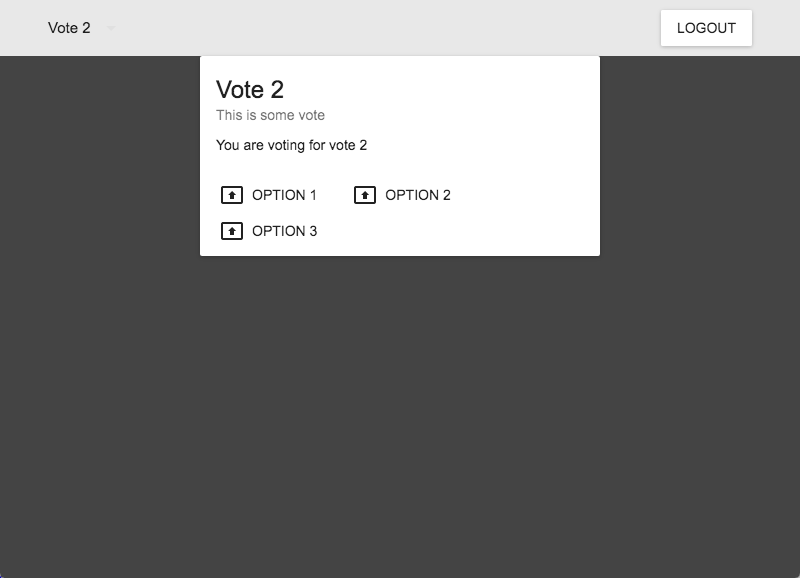
\includegraphics[width=0.9\textwidth]{screenshots/screen-vote-voting}
        \caption{The voting screen for the desktop application.}
        \label{fig:registration}
    \end{figure}
\end{centering}

\newpage
\printbibliography[heading=bibintoc]
\end{document}